\documentclass{article}
\usepackage[utf8]{inputenc}
\usepackage[margin = 0.8in]{geometry}
\usepackage{graphicx}
\usepackage{amsmath, amssymb}
\usepackage{caption}
\usepackage{subcaption}
\usepackage{multirow}
\usepackage{multicol}
\usepackage{booktabs}
\usepackage{bm}
\setlength{\columnsep}{.75cm}
\usepackage{float}
\usepackage{graphicx}
\usepackage{stfloats}
\usepackage{hyperref}
\graphicspath{ {./images/} }
\setcounter{MaxMatrixCols}{15}

\renewcommand\refname{References}
\restylefloat{table}


\title{Autonomous Operation for Last-Mile Food, Grocery, and Goods Delivery on a Suburban Sidewalk\\
\vspace{5mm}
\large RBE550-Spring 2022 }
\author{Keith Chester, Bob DeMont}
\date{May 2, 2022}

\begin{document}
\maketitle

\begin{multicols}{2}
\section*{Abstract}
The purpose of the project is to simulate successful autonomous navigation of a delivery robot along sidewalks in a busy suburban environment from store to a delivery address on ground level.  It demonstrates global planning for high-level route planning with a hand-off to a local planner for obstacle avoidance.

\section*{Background}
Last mile delivery has been a growing issue with the increase in e-commerce over at least the last 8 years with each year growing from 15-30\% from the year before \cite{Ecom}.  Since much of this final delivery is accomplished via vehicles, the has been an accompanying call for reduced emissions.  A McKinsey study estimates that this could lead to a 25\% increase in CO2 emission in cities \cite{Emiss}.  Most recently, the COVID pandemic with its isolation mandates have led to even greater demand for delivery of not only goods but also everyday essentials such as meals, groceries, and prescription medicine.  This needed to be accomplished with minimal human contact while fewer humans were available due to quarantines and employee availability.  For grocery delivery, the need for fastest route planning is also necessary due to the presence of perishables and temperature sensitive cargo - or, in other words, people prefer their meals hot and their frozen goods cold. Cheng et al \cite{Mcheng} have shown efficient curb detection to set the limits of the robot's path.

\section*{Goals}
Our goal is to create planning and execution algorithms to permit autonomous navigation and avoidance of both static (dumpsters, trashcans, traffic cones, garbage cans and garbage bags) and dynamic obstacles (people, cars) while following sidewalk rules (staying on the sidewalk and crossing at crosswalks etc).

\subsection*{Robot Choice}
\textbf{Design} After research of the prevailing designs for this type of application, we've settled on a non-holonomic 6 wheeled robot using skid steering. It uses a simulated GPS sensor for a pre-determined, global path plan and simulated LIDAR for more specific localized obstacle avoidance during operation. \\
\vspace{2mm}\\
\noindent \textbf{Kinematics.} The kinematics for the robot are modeled on a diwheel design.  This resulted in the following state transition functions:
\begin{equation}
\begin{split}
\dot{x}&=r(u_r+u_L)\cos\theta\\
\dot{y}&=r(u_r+u_L)\sin\theta\\
\dot{\theta}&=\frac{r}{L}(u_r-u_L)\\
\end{split}
\end{equation}
\noindent where$ L$ is the distance between the wheels, in our case .66 meters,  $r$ is the radius of the wheels (.1m) and $u$ is the rotational velocity of wheels of the left and right sides.\\

\begin{figure}[H]
   \centering
    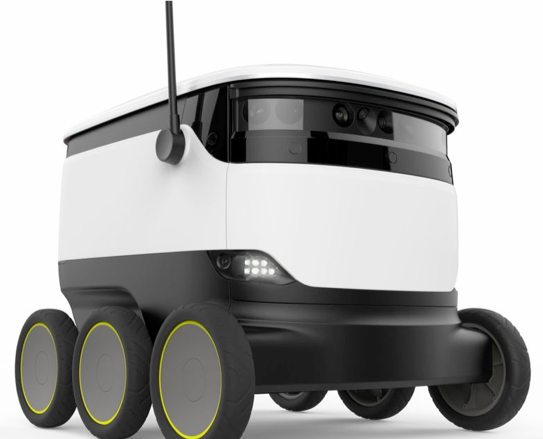
\includegraphics[width = .75\columnwidth]{figures/delbot.png}
     \label{fig:delbot}
     \caption{Robot Model}
\end{figure}
\section*{Methods}
\noindent \textbf{Global map}.  The overall map is overlayed with designated waypoints which may be turns, crosswalks, or delivery addresses.  This generates a master map of feasible routes which is translated into a graph representation for optimal global route selection via a number of algorithms.  Below demonstrates the environment map as well as the waypoint/graph representation.\\
\begin{figure}[H]
   \centering
    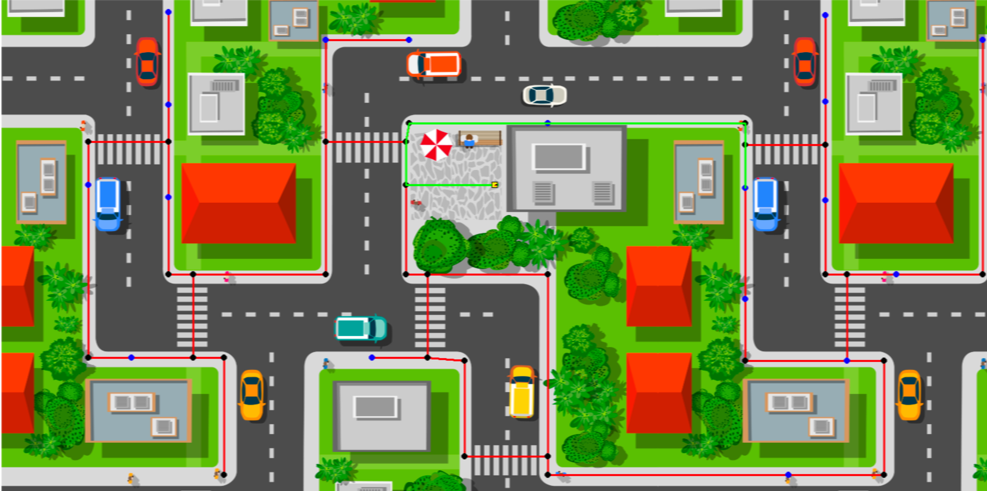
\includegraphics[width = 1\columnwidth]{figures/routemap.png}
     \label{fig:routemap}
     \caption{Global Route Map}
\end{figure}
\noindent \textbf{Global Planner} We selected a simple A* algorithm for global path selection.  With a given route map, no complexity is involved.  Each path segment returned represents a leg of the global route between waypoints.  \\

\noindent \textbf{Local Planner} Each leg of the global path is then, in turn, passed to the local planner which uses a slightly more complex A* to account for collision detection and reject off-limits positions.  
\begin{figure}[H]
   \centering
    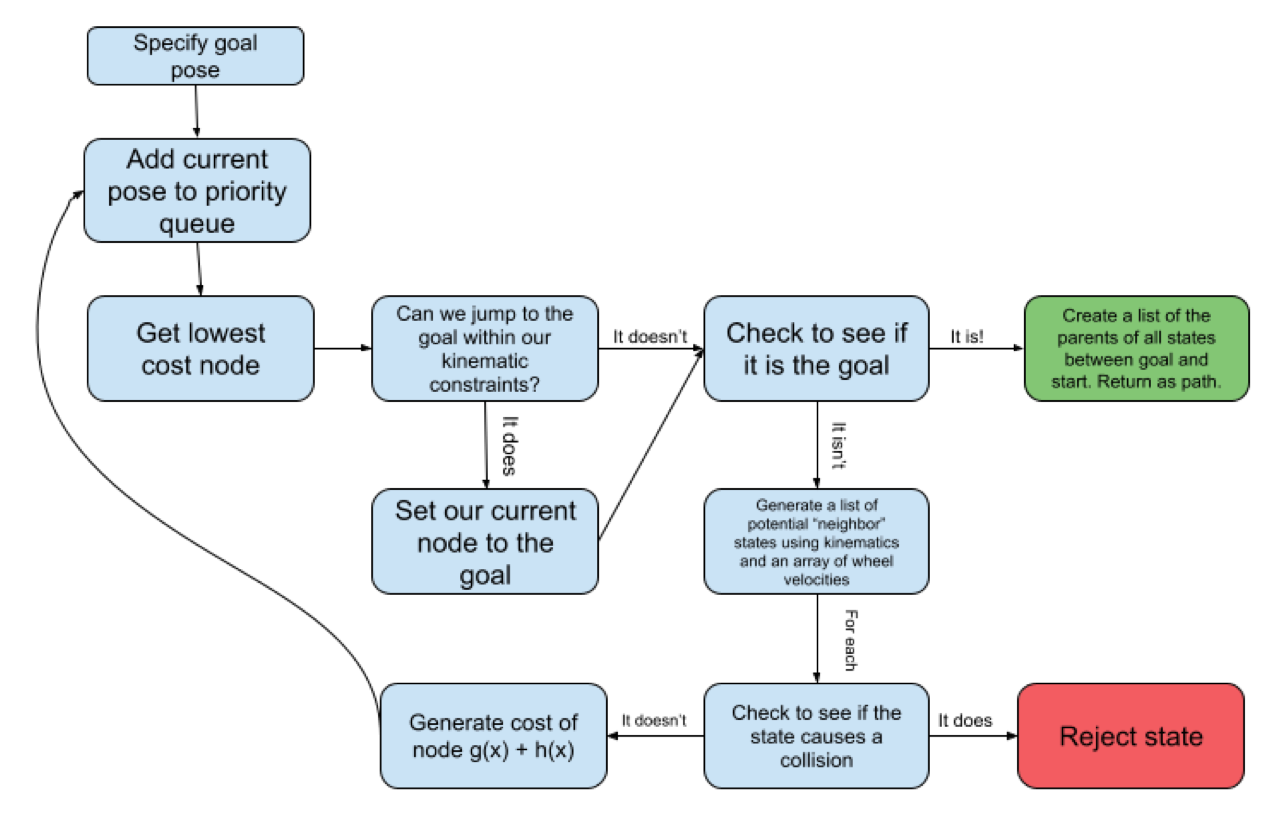
\includegraphics[width = 1\columnwidth]{figures/astar.png}
     \label{fig:astar}
     \caption{A* Local Planner}
\end{figure}

\noindent \textbf{Asynchronous Planner}. An asynchronous planner was created to speed presentation times.  This permits next step, local path planning while the robot is completing its current local leg.  \\
\noindent Keith- add anything you want here or delete if the others cover it enough.\\

\noindent \textbf{Simulation}. For simulating the environment we chose to use Pygame to capitalize on the collision detecting built into the sprite class.  A mask of the off-limits areas creates the curb and building limits for our robot's movement. We use the the alpha layer of the sprites for pixel-by-pixel comparisons- useful for tight transitions between obstacles..\
\begin{figure}[H]
   \centering
    
\includegraphics[width = 1\columnwidth]{figures/mask.png}
     \label{fig:mask}
     \caption{Initial Collision Map}
\end{figure}

\noindent \textbf{Stationary Obstacles}. In addition to off limits areas (buildings and streets-less-crosswalks) we place other obstacles into the environment.  These took the form of trashcans, trash bags, bicycles, dumpsters and traffic cones.  These obstacles were, of course, unknown to the global planner but register for the local planner as it seeks a path with obstacle avoidance.  As part of the obstacle set, moving vehicles will be included on the roads to be avoided at the crosswalks.
\begin{figure}[H]
   \centering
    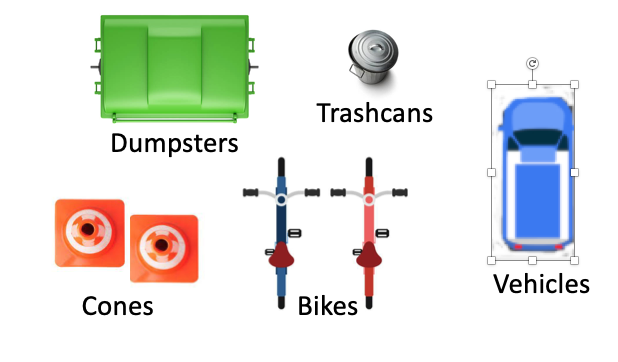
\includegraphics[width = 1\columnwidth]{figures/obstacles.png}
     \label{fig:obstacles}
     \caption{Obstacle Set}
\end{figure}
\noindent \textbf{Moving Obstacles}. Random vehicle deigns are generated with random speeds between 6 and 12 m/sec along 4 set routes:these constitute our moving obstacles. For these, we simulate sensing the distance of an approaching vehicle.  If it is inside a safe movement distance the robot waits before initiating movement along the planned local route. When "the coast is clear", we initiate movement again.  If the robot is already in the crosswalk, perhaps delayed by planning around a crosswalk obstacle, the car has to stop to honor crosswalk rules.  After the robot clears, the vehicle proceeds again.\\

\section*{Results}
\textbf{Planners}. We tested in phases as we constructed.  The global planner worked flawlessly  as the first simulation part tested after creation of the environment and global network.  No difficulties were encountered.  The local planner required some tuning of state variables to simply the question of "have we been here before?".  Initially small state variations, which were essentially the same state, registered as different states and bogged calculations.  As we incorporated some rounding, performance improved. To smooth paths further, we borrowed a repulsive concept from APF and incorporated a near-the-obstacle penalty into the heuristic for search node generation.  Integrating global and local planners worked well.  The global path handoff was successful and the local search found a fairly direct path.  \\
\noindent \textbf{Stationary Obstacles}.  Incorporating obstacles brought to light some interesting challenges.  If the obstacle happened to be covering the waypoint, it was impossible for the local search to complete.  One strategy might have been to abandon the immediate waypoint after a certain number of attempts and try to proceed to the next waypoint.  We chose instead to insure obstacles weren't directly on top of waypoints.  After that, we were able to navigate around all obstacles.  Some took longer that others depending on the collision space, but all eventually solved.  \\
\noindent \textbf{Moving obstacles}.  Moving obstacles are successfully detected as approaching and the robot is locked out of proceeding until the car passes.  If the car comes near the crosswalk while the robot is already in the crosswalk and negotiating an obstacle, the car stops according to crosswalk rules and proceeds when the robot clears the crosswalk.
\begin{figure}[H]
   \centering
    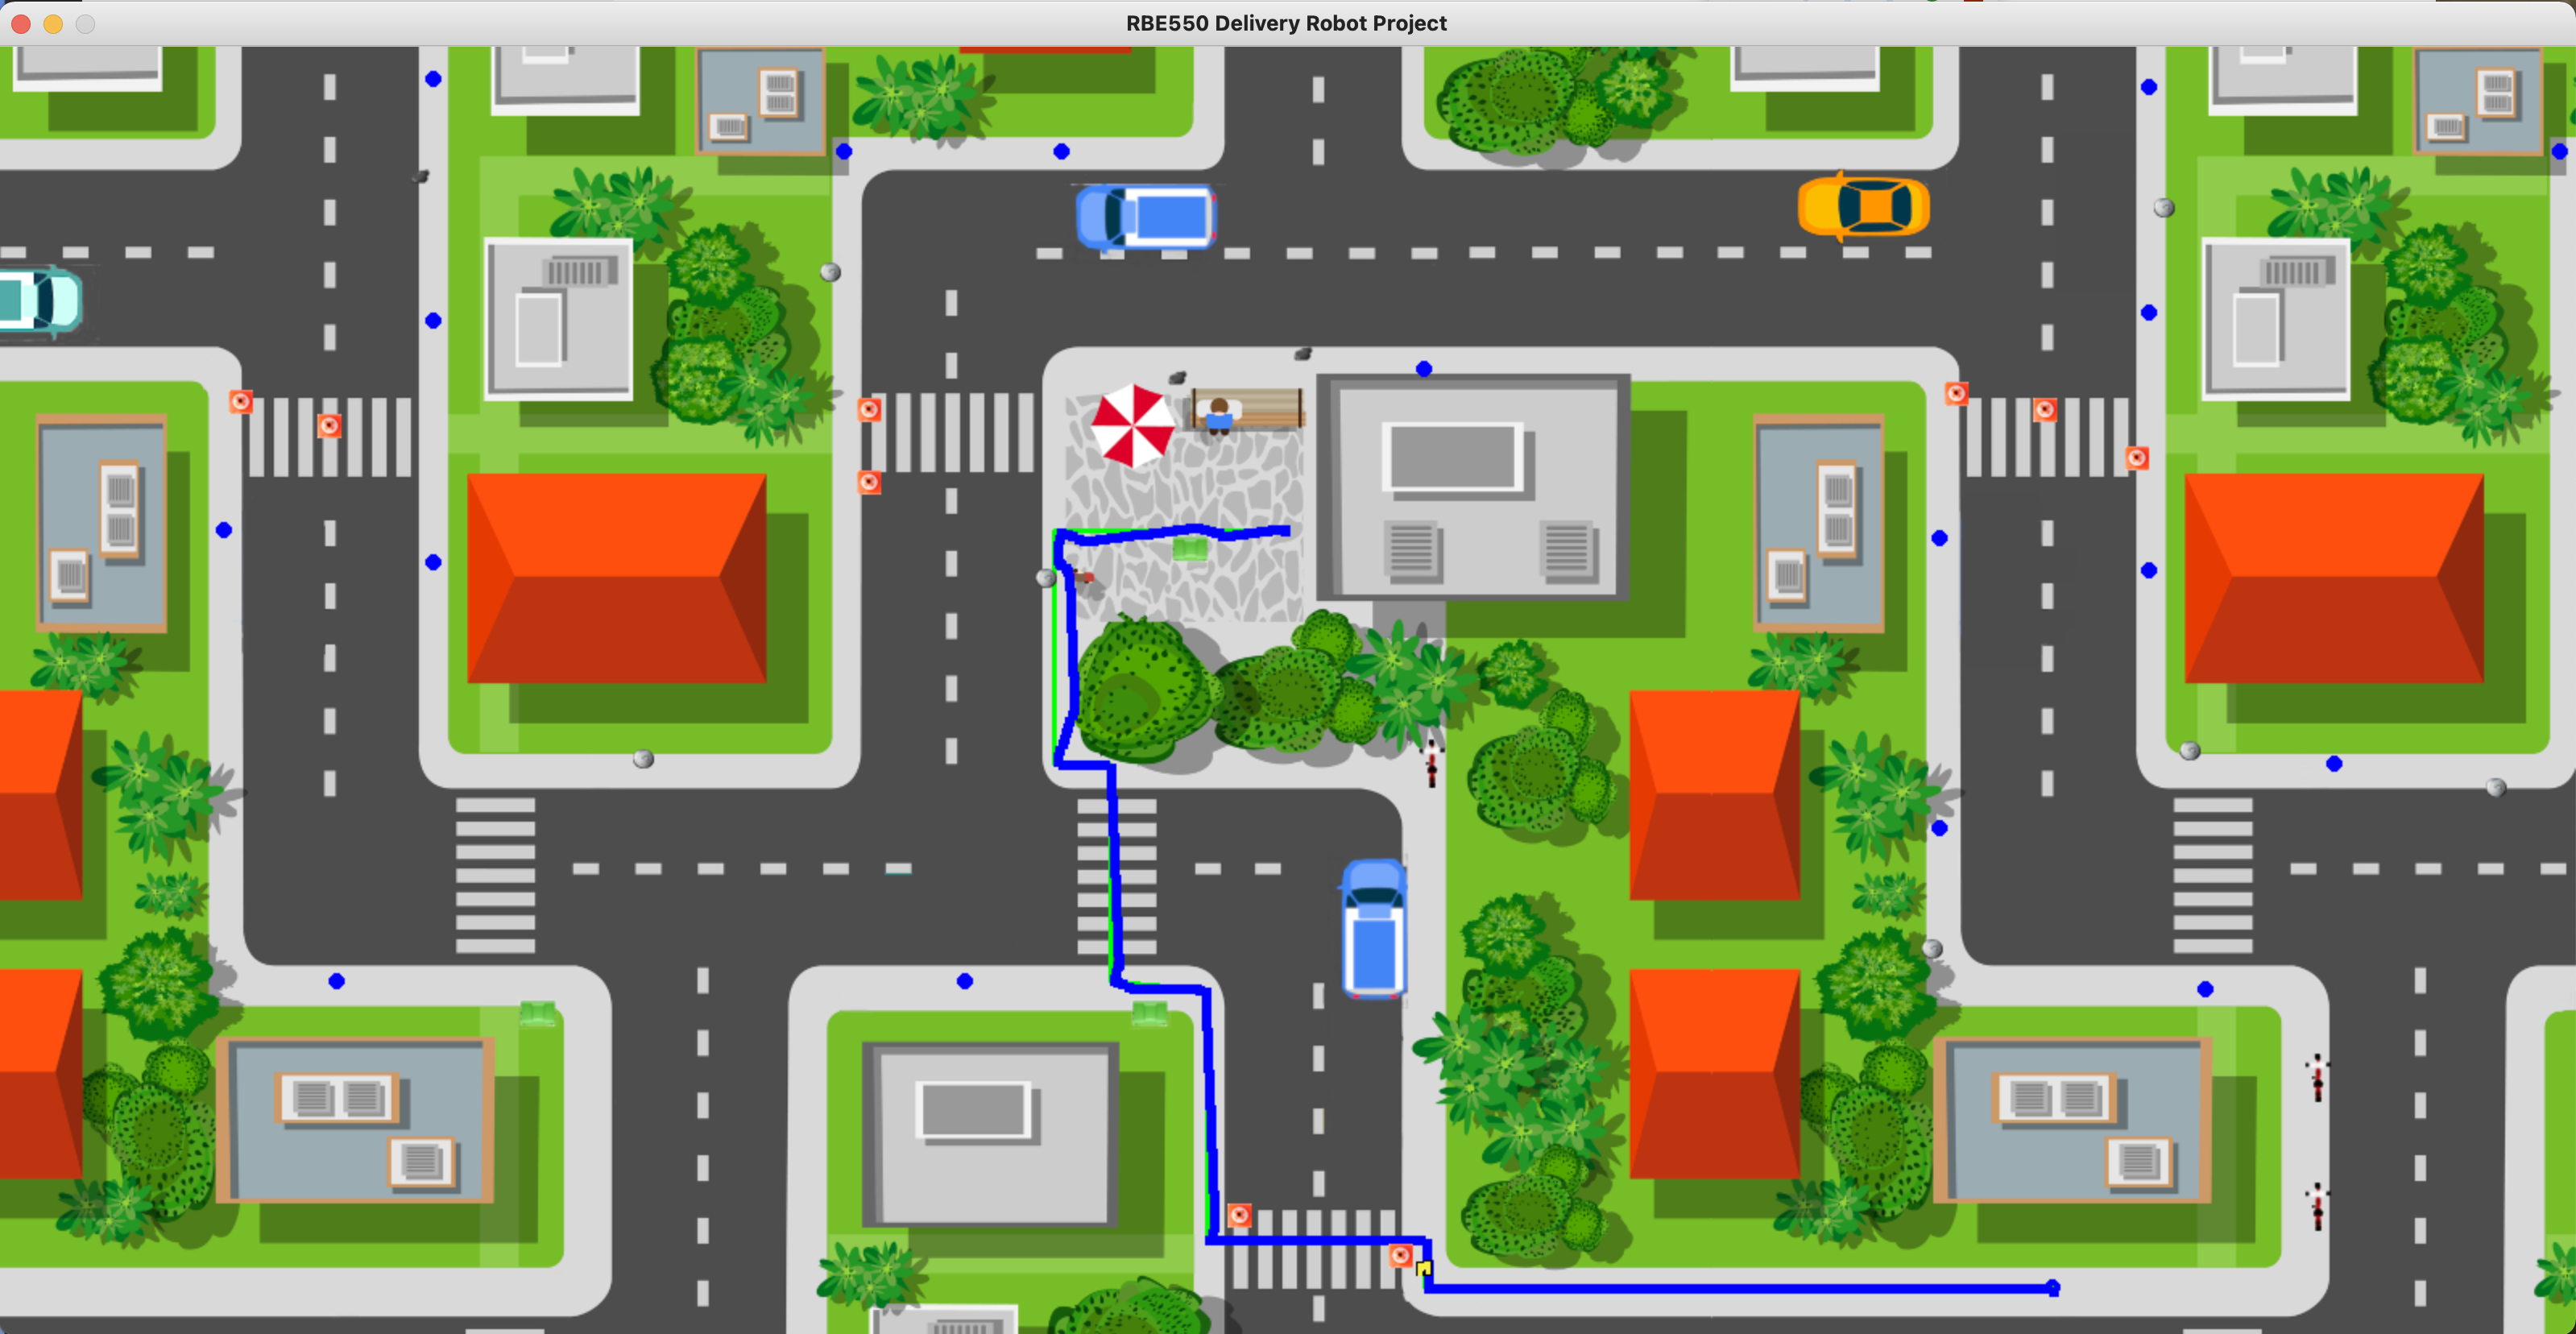
\includegraphics[width = 1\columnwidth]{figures/running.png}
     \label{fig:running}
     \caption{Simulation Running}
\end{figure}

\section*{Conclusions}
\noindent Our technique of integrating the higher level global path plan for route planning with a lower level, local planner for collision avoidance allowed us to successfully navigate a suburban sidewalk strewn with obstacles for last mile delivery of groceries or packages.  Incorporating a small repulsive force in our local planner search heuristic allowed us to generate smoother paths through obstacle avoidance rather than obstacle handling.  

\section*{Further Opportunities}
\noindent Further opportunities exist to explore algorithmic approaches to solving the problem of when an obstacle is on top of a waypoint.  We solved by  insuring the robot could get "close enough" the the waypoint to begin the next leg.  We also considered the generation of two to three random destinations for the robot to deliver on the same route.  This adds complexity to the global planner to deliver an optimized route through 2-3 destinations.  Thankfully the delivery capacity in this case is small enough to avoid a complex "Travelling Salesman" problem.
\label{References}

\bibliographystyle{abbrv}
\begin{thebibliography}{10}
\bibitem{Ecom} https://www.statista.com/statistics/379046/worldwide-retail-e-commerce-sales/
\bibitem{Emiss}https://www.mckinsey.com/industries/travel-logistics-and-infrastructure/our-insights/efficient-and-sustainable-last-mile-logistics-lessons-from-japan
\bibitem{Kocs}
M. Kocsis, J. Buyer, N. Sußmann, R. Zöllner and G. Mogan, "Autonomous Grocery Delivery Service in Urban Areas," 2017 IEEE 19th International Conference on High Performance Computing and Communications; IEEE 15th International Conference on Smart City; IEEE 3rd International Conference on Data Science and Systems (HPCC/SmartCity/DSS), 2017, pp. 186-191, doi: 10.1109/HPCC-SmartCity-DSS.2017.24.
\bibitem{Mcheng}
M. Cheng, Y. Zhang, Y. Su, J. M. Alvarez and H. Kong, "Curb Detection for Road and Sidewalk Detection," in IEEE Transactions on Vehicular Technology, vol. 67, no. 11, pp. 10330-10342, Nov. 2018, doi: 10.1109/TVT.2018.2865836.
\bibitem{Construct} https://www.theconstructsim.com/
\bibitem{ROS-Docker} http://wiki.ros.org/docker/Tutorials/Docker
\bibitem{Thackston} https://www.allisonthackston.com/articles/vscode-docker-ros2.html



\end{thebibliography}
\pagebreak
\section*{Appendix-Contributions}
\noindent \textbf{Keith Chester}-Keith did most of the Python coding for the team.  We both participated in debugging efforts and review and finalization of the submissions and feel the workload was evenly distributed.
\bigskip

\noindent \textbf{Bob DeMont}-Bob took care of the fiddly work of obtaining graphics, sorting out coordinates, tuning parameters, sorting out car movements and drafting the presentations and report.  We both participated in debugging efforts and finalization of the submissions and feel the workload was evenly distributed.
 
 

\end{multicols}

\end{document}
